\section{Experimental}

Focus areas: Contaminants from Chromium, Titanium, Iron.


\subsection{Samples}

4 Samples: All polished and etched on top

Chromium contaminated, less than 10$^13$ cm$^-3$

Boron and Phosphorus equally distributed around 10$^16$ cm$^-3$.

Regular MC solar grade sample

Pure Si sample (FZ?)

\subsection{Setup}


\begin{figure}[H]
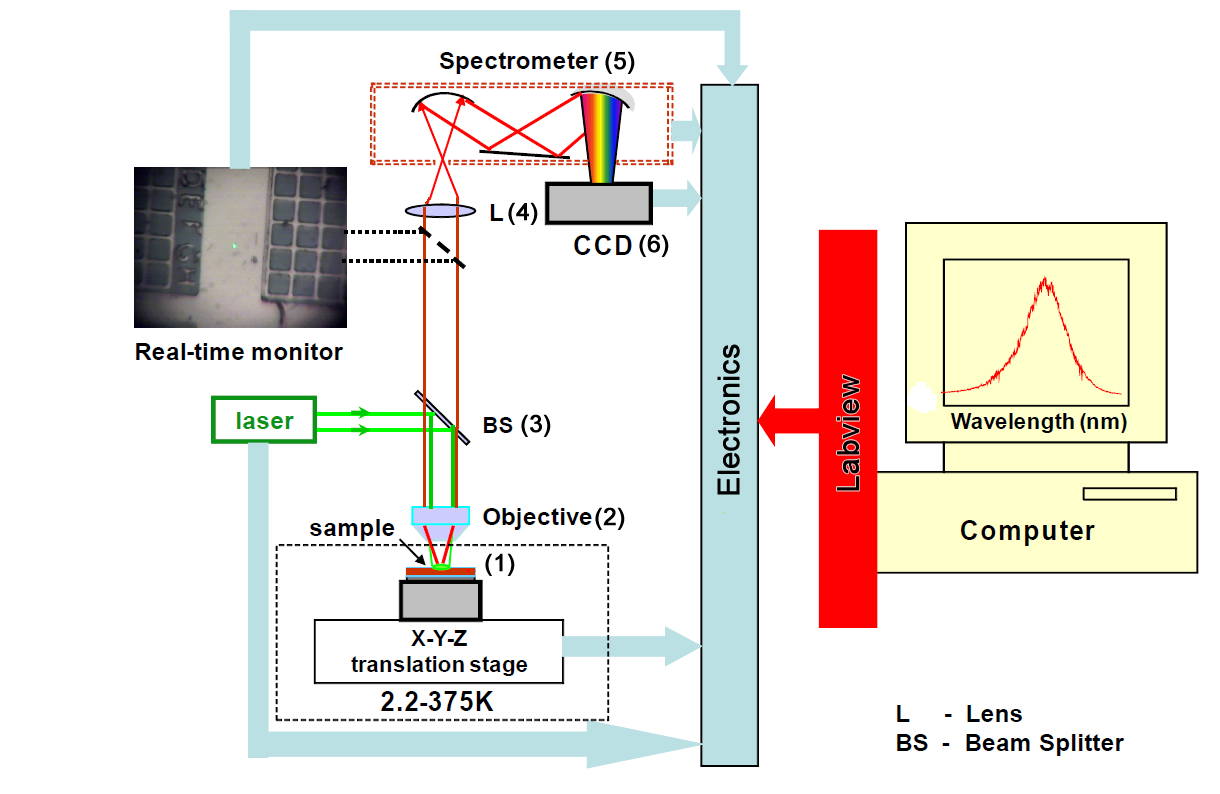
\includegraphics[width=\columnwidth]{lab_setup}%
\caption{Lab setup}%
\label{fig:lab_setup}%
\end{figure}



\begin{table}[H]
\centering
\begin{tabular}{|c|c|c|c|}
\hline
\textbf{\#} & \textbf{Part} & \textbf{Product \#} & \textbf{Manufacturer} \\
\hline
1 & Cryostat & Janis ST-500 & Janis Research Company \\ \hline
2 & Objective & NT56-982 & Edmund Optics \\ \hline
3 & Beam splitter & BS017 & Thorlabs \\ \hline
4 & Lens & ACN127-020-B & Thorlabs \\ \hline
5 & Spectrometer & iHR550 Imaging Spectrometer & Horiba Scientific \\ \hline
9 & Kamera & InGaAs Spectroscopy CCD & Andor Technology \\ \hline
\end{tabular}
\caption{Lab setup optical components}
\label{tab:lab_setup}
\end{table}

\subsection{Pumping wavelength}

Pumping light needs to have enough energy to fill all available states in the crystal lattice, in order to detect defects and impurities. For silicon, which has a bandgap of around 1.1eV, has most impurity/defect bands below the bandgap. In order to fill these states, the pumping wavelength should be below 1125nm, which corresponds to energies just over 1.1eV.

Silicon has different absorption lengths for different wavelengths. For 1125nm, the absorption depth is nearly 200~$�$m \cite{laserdybde}. Compared to absorption for 532nm, 1125nm reach 200 times deeper into the sample.

Absorption length of about 1~$�$m for 532 nm laser, means that iron precipitates deeper in the sample won't be detected \cite{gundel09}. This limitation might be overcome by an excitation laser with a longer wavelength and absorption length in silicon. \cite{lee09} report that small angle grain boundaries in multicrystalline silicon of 1$^\circ$-1.5$^\circ$ show D3 and D4 lines, while 2$^\circ$-2.5$^\circ$ show D1 and D2 lines. Comparing to data from electron beam induced current measurements show D1 and D2 lines to be correlated with shallow levels, while D3 and D4 appear in both shallow and deep levels \cite{lee09}.

A pumping wavelength of 800 nm is chosen for excitation. This corresponds to an absorption depth of 12~$�$m in silicon. With a larger wavelength, it would be invisible to the naked eye, and make it much more difficult to align the setup, and make sure nothing is blocking the pathway. In the case of an imperfect filter in front of the spectrometer, 800nm (1.55eV) and the second order diffraction maxima at 1600~nm (0.775~eV) would be outside the most interesting wavelengths from silicon luminescence (see table \ref{energy_bands}).

\subsection{Spot size}

Having a small diameter on the pumping laser allows for a high resolution of characteristics on the sample. In an iron contaminated sample, \cite{gundel09} show that at some distinct spots of a size between 1$�$m and 4$�$m, the band to band photoluminescence peak is particular low at spots with iron precipitates. 

A large electron hole droplet could overshadow characteristics from impurities in the sample. \cite{satoshi04} show that electron hole droplets become more intense for a smaller volume, with a silicon nanolayer smaller than the absorption depth of the laser. \cite{satoshi04} used a 488nm pumping laser with 1,5$�$m diameter, on silicon nanolayer thickness of 50nm and 340nm. For the 50nm layer, \cite{satoshi04} observed a large electron hole droplet, even for small pumping intensities, with the same amount of photo excited carriers per volume as for the 340nm layer. Assuming that a small volume give rise to a larger electron hole droplet, it would be a limiting factor for the spot size and pumping wavelength.

For the setup given here, the spot size is around 2~$�$m.

\subsection{Laser intensity}

With a large pumping intensity, an electron hole droplet become visible in the specter around 1.08eV in bulk silicon \cite{hammond75}. \cite{satoshi04} show that electron hole droplets occur at weak excitations (0.75mW) and even at high temperatures for a silicon nanolayer of 50nm. For thickness of 340nm, the electron hole droplet show up at pumping intensity of 3mW and above, and the intensity of the electron hole droplet grow larger than for the free exciton at 15mW. This electron hole droplet is not wanted, as it can mask characteristic photoluminescence from impurities.

With a larger pumping intensity, the impurity photoluminescence would in some cases also increase. Photoluminescence from chromium bound with a boron atom is known to increase linearly with laser power \cite{conzelmann82,conzelmann83}, and would be easier to detect at a higher pumping intensity.